%!TEX root = ../main.tex
% Chapter 1

%\chapter{background}
\chapter{Introduction and Problem Statement}
The purpose of this assignment is to design, simulate and implement a PI controller to compensate a DC motor using a microcontroller. The implementation will be assessed by means of a report in accordance with ECSA ELO 2, as part as the following milestones:
\begin{description}
	\item[Milestone 1] Characterisation of a DC motor
	\item[Milestone 2] Mathematical modelling and simulation of the DC motor
	\item[Milestone 3]Controller design and simulation of closed loop system
	\item[Milestone 4] Practical demonstration of controller design
	\item[Milestone 5]  Final report
\end{description}
The first milestone was completed successfully earlier in the semester and the lab report is included in appendix A. 







\chapter{Literature Study}
\section{Modeling the DC Motor}
According to the Prescribed textbook\cite[p.160]{dorf2011modern}: \\ \blockquote{\emph{Time constant}\\ The time interval necessary for a system to
change from one state to another by a specified percentage. For a first order system, the time constant is
the time it takes the output to manifest a 63.2\%
change due to a step input.}

\section{Simulatong the system}
\blockquote{Simulink, developed by The MathWorks, is an environment for multidomain simulation and
Model-Based Design for dynamic and embedded systems. It provides an interactive
graphical environment and a customizable set of block libraries that let you design, simulate,
implement, and test a variety of time-varying systems, including communications, controls,
signal processing, video processing, and image processing.
With Simulink, you build models by dragging and dropping blocks from the library browser
onto the graphical editor and connecting them with lines that establish mathematical
relationships between blocks. You can set up simulation parameters by double clicking the
blocks.\\
\cite[p.4]{li2008simulink}}




\chapter{Modeling}
In this section the characteristics of the DC motor need to be interpreted in a way that allows an appropriate controller to built around it. The List of all the measured parameters, and methods are included in the ``One page Experiment design'' included in \hyperref[apx:A]{Appendix A}.Since the specification only requires a first order model of the motor, and since the mechanical time constant overwhelms the electrical time constant, the mechanical time constant is the only parameter necessary to meet the specifications.
\section{Measuring the Mechanical Time constant}
With regards to the definition of a time constant as discussed in the Literature study, the time constant of the DC motor was calculated by plotting the rotational velocity of the over time after shutting off the power source. Refer to Figure~\ref{fig:shutoff}
These Measurements were taken by connecting the Tachometer to the PicoScope and recording the values into a .csv file. The Data was prepared for plotting in the following ways:
\begin{itemize}
	\item The time stamps were offset so that the shutoff occurred at $t=0$ 
	\item The tachometer gave a reading 360mV when the speed was 0 RPM, so the Y axis was offset accordingly
	\item The Data was smoothed using an average filter. See python script in \hyperref[apx:B]{Appendix B}
\end{itemize}

\begin{figure}[h]
    \myfloatalign
    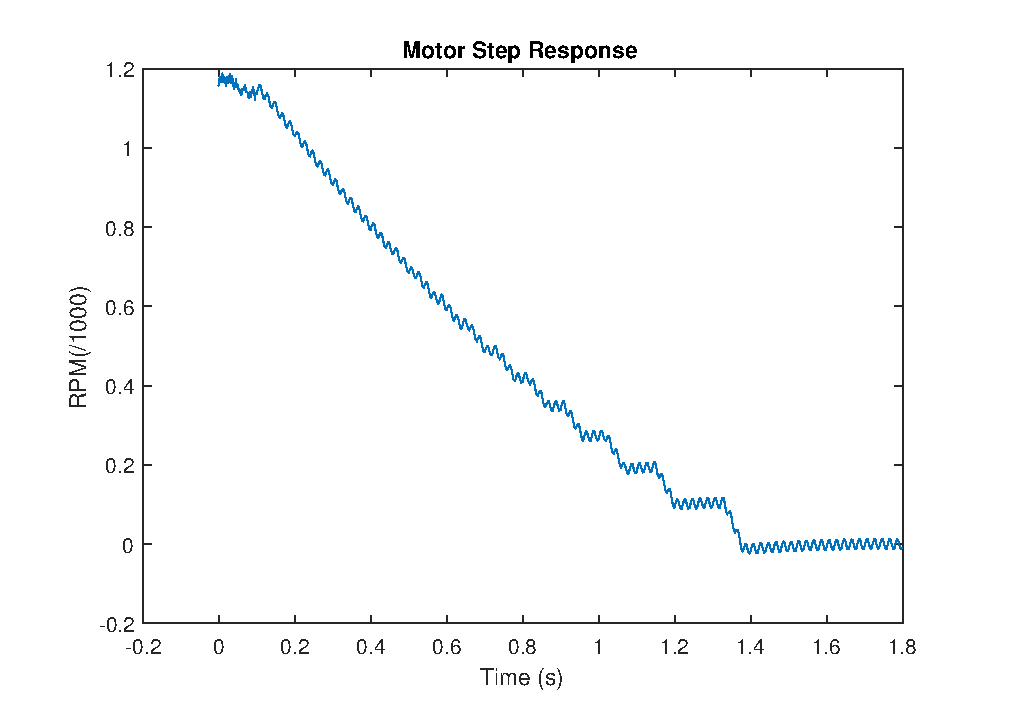
\includegraphics[width=1.2\textwidth]{gfx/Motor_shutoff} %can also be placed in images/example
    \caption{Time Response of the DC motor}
    \label{fig:shutoff}
\end{figure}
From the representation of the data in Figure~\ref{fig:shutoff}, it can be measured that the motor took Approximately 0.77 seconds to reach a speed of 440RPM, A value 63\% from the steady state value. The mechanical time constant $\tau_\ell$ is given by:
\begin{equation}
	\tau_\ell = 0.77s
\end{equation}
\section{Determining K and comparing the model with the results}
Having measured the time constant, the time domain model of the DC motor is in the form:
\begin{align}
	\dot{\omega}(t) &= Ke^{\frac{t}{\tau_\ell} }
\end{align}
Using the value calculated for $\tau_\ell$ and choosing K by means of trial and error, the following model was found to be reasonably close to the measured response:
\begin{align}\label{eq:1}
	K &= 1.2\\
	\dot{\omega}(t) &= 1.2e^{\frac{t}{0.77} }\\
	G(s) &= \frac{1.2}{0.77s+1} 
\end{align}
Refer to Figure~\ref{fig:shutoff_vs_model}, where the time domain model is compared to the measured results. It must be noted that, at this stage in the practical process, the motor was modeled as a function of the input voltage, which was in the order of 0-400V. This model, therefore represents the response to a 400V step in input. It was later found that the motor must be compensated using a duty cycle. Finally, both the reference speed and tachometer output are given in the form:
\begin{align}
1 RPM &= 1mV	
\end{align}
These considerations obviously render the above transfer function unusable (since a plant input in the order of 100 corresponds to an output in the order of 1) and the gain K, must be adjusted before designing the PI controller. It was found that lowering the gain by a factor of 100 yielded an appropriate plant transfer function. By definition, the time constant stays unchanged, regardless of the gain.The transfer function on which the PI controller will be based is therefore given by:
\begin{align}
	\label{eq:motortf}
	G(s) &= \frac{0.012}{0.77s+1} 
\end{align}



\begin{figure}[h]
    \myfloatalign
    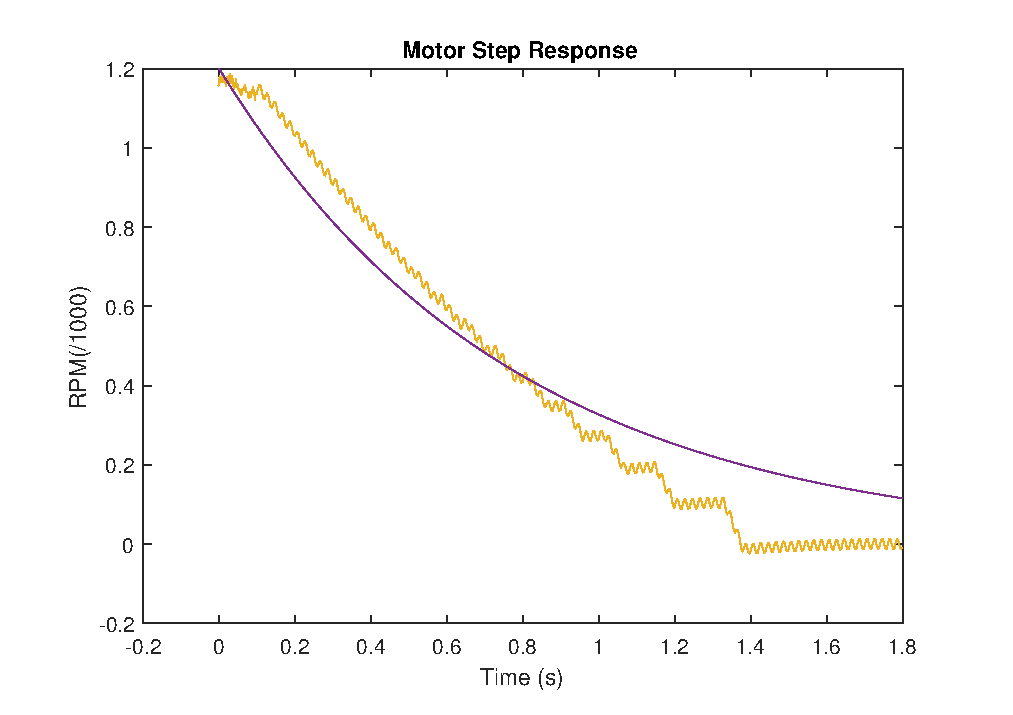
\includegraphics[width=1.2\textwidth]{gfx/Motor_shutoff_vs_Time_domain_model} %can also be placed in images/example
    \caption{Simulation of the time domain model compared with Laboratory results}
    \label{fig:shutoff_vs_model}
\end{figure}
\section{Designing the PID}
The following table shows the specifications that the system must adhere to:

\begin{table}[h]
\centering
\caption{Specifications}
\label{tbl:spec}
\begin{tabular}{llll}
\cline{1-2}
\multicolumn{1}{|l|}{\textbf{Parameter}}      & \multicolumn{1}{l|}{\textbf{Maximum Value}} &  &  \\ \cline{1-2}
\multicolumn{1}{|l|}{Steady state error}    & \multicolumn{1}{l|}{1\%}                   &  &  \\ \cline{1-2}
\multicolumn{1}{|l|}{Percent Overshoot(P.O.)} & \multicolumn{1}{l|}{10 \%}                       &  &  \\ \cline{1-2}
\multicolumn{1}{|l|}{Settling time} & \multicolumn{1}{l|}{<2s}                       &  &  \\ \cline{1-2}
                                              &                                             &  & 
\end{tabular}

\end{table}
The transfer function for a PI controller in General is given by:
\begin{equation}\label{eq:2}
	G_{c}(s) = K_{c}+ \frac{K_{i}}{s}
\end{equation}
The equations for Percent overshoot and settling time are given by:
\begin{align} \label{eq:poform}
P.O. &= e^{\left( \frac{-\pi\zeta}{\sqrt{1-\zeta^2}}\right)}
\end{align}
\begin{align}\label{eq:tsform}
T_s &= \frac{4}{\zeta\omega_n}
\end{align}

Furthermore, $\zeta$ and $\omega_n$ can be used to define a desired characteristic equation in the form:

\begin{align} \label{eq:4}
Q(s) &= s^2 + 2\zeta\omega_ns + \omega_n^2
\end{align}

The PI controller design can be summed up as the reconciliation of the desired characteristic equation \ref{eq:4} with the characteristic equation of the system, which is given by:
\begin{align}\label{eq:5}
Q(s) &= G(s)G_c(s) + 1 
\end{align}
With respect to the equations \ref{eq:motortf} and \ref{eq:2}\\
This design is described in the next section.


%----------------------------------------------------------------------------------------

\chapter{Controller Design}
\section{Determining $\zeta$ and $\omega_n$}
Substituting the P.O from Table~\ref{tbl:spec} and solving equation~\ref{eq:poform} yields:
\begin{align}
	\label{eq:zetacalc}
	P.O. &= e^{\left( \frac{-\pi\zeta}{\sqrt{1-\zeta^2}}\right)}\\
	0.1 &= e^{\left( \frac{-\pi\zeta}{\sqrt{1-\zeta^2}}\right)}\\
	\zeta &= 0.5911 \text{ solved numerically} 
\end{align}
Substituting the result of Eq~\ref{eq:zetacalc} and the settling time from Table~\ref{tbl:spec} into eq~\ref{eq:tsform} yields:
\begin{align}
	\label{eq:omegacalc}
	2 &= \frac{4}{\zeta\omega_n} \rvert_{\zeta = 0.5911}\\
	\omega_n &= 3.384
\end{align}

\section{solving for $K_p$ and $K_i$}
Reconciling the compensated transfer function and desired transfer function yields:
\begin{align}
	\label{eq:kpkichar}
Q(s) &= 1 + G_c(s)G(s) \\
Q(s)&= s^2 + 2\zeta\omega_ns + \omega_n^2\\
Q(s) &= s^2 + s(1.298 + 0.012K_p) + 0.012K_i 
\end{align}

By the principle of superposition:
\begin{align}
2\zeta\omega_n &= 1.298 + 0.012K_p \\
\omega_n^2 &= 0.012K_i 
\end{align}
\begin{align}
	\label{eq:}
	K_p &= 255.155\\
	K_i &= 954.288\\
\end{align}
\emph{Note: the values of $K_p$ and $K_i$ seem very high, but this is by design, since the PI controller must have a very high gain, converting an error input in the order of 1V to an output in the order of 100\% }
\section{testing the results}
Figure~\ref{fig:theoplot} was plotted to confirm the calculations. The result was very close to the specification, in the simulation, these results will be tuned, since the specifications are given as upper limits.

\begin{figure}[h]
		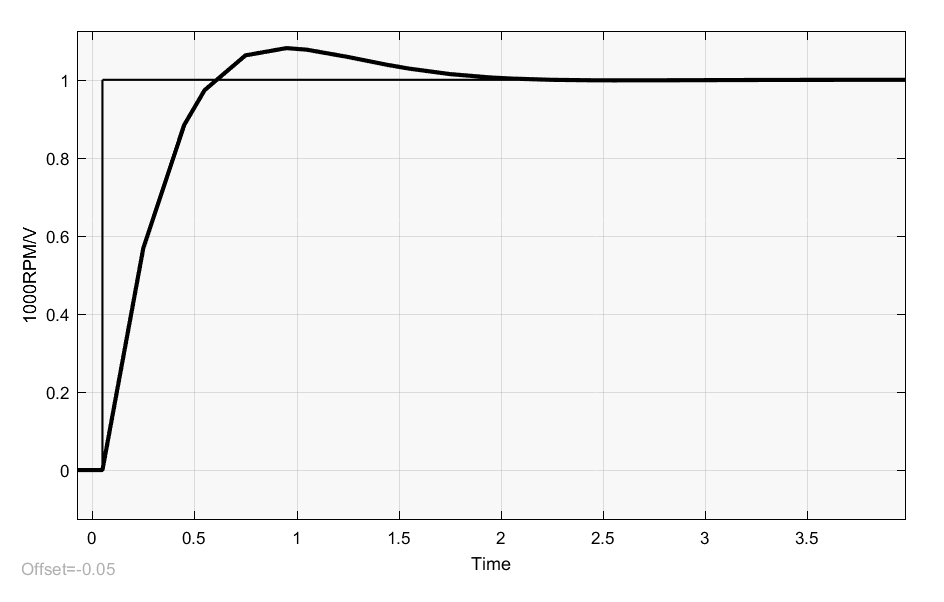
\includegraphics[clip,width=0.7\textwidth]{gfx/calc_plot}%
		\caption{Plot of the transient response of the Caculated system}
\label{fig:theoplot}
\end{figure}


Table~\ref{tbl:theospec} Compares the specification to the theoretical result of the calculated parameters:

\begin{table}[h]
\centering
\caption{Theoretical Results}
\label{tbl:theospec}
\begin{tabular}{llll}
\cline{1-2}
\multicolumn{1}{|l|}{\textbf{Parameter}}      & \multicolumn{1}{l|}{\textbf{Value}} &  &  \\ \cline{1-2}
\multicolumn{1}{|l|}{Steady state error}    & \multicolumn{1}{l|}{0\%}                   &  &  \\ \cline{1-2}
\multicolumn{1}{|l|}{Percent Overshoot(P.O.)} & \multicolumn{1}{l|}{10.5 \%}                       &  &  \\ \cline{1-2}
\multicolumn{1}{|l|}{Settling time} & \multicolumn{1}{l|}{2.2s}                       &  &  \\ \cline{1-2}
                                              &                                             &  & 
\end{tabular}

\end{table}


\chapter{Controller Simulation}
Simulink automates most of the simulation process. Figure~\ref{fig:simblockdiagram} Shows the simple simulation. The simulation was also used to tune the Parameters calculated in the previous section to be well within the specifications. These tuned parameters were implemented using the controller.The parameters after the tuning process are given by:
\begin{description}
	\item[$K_p$] 300 
	\item[$K_i$] 800
\end{description}
\begin{figure}[h]
	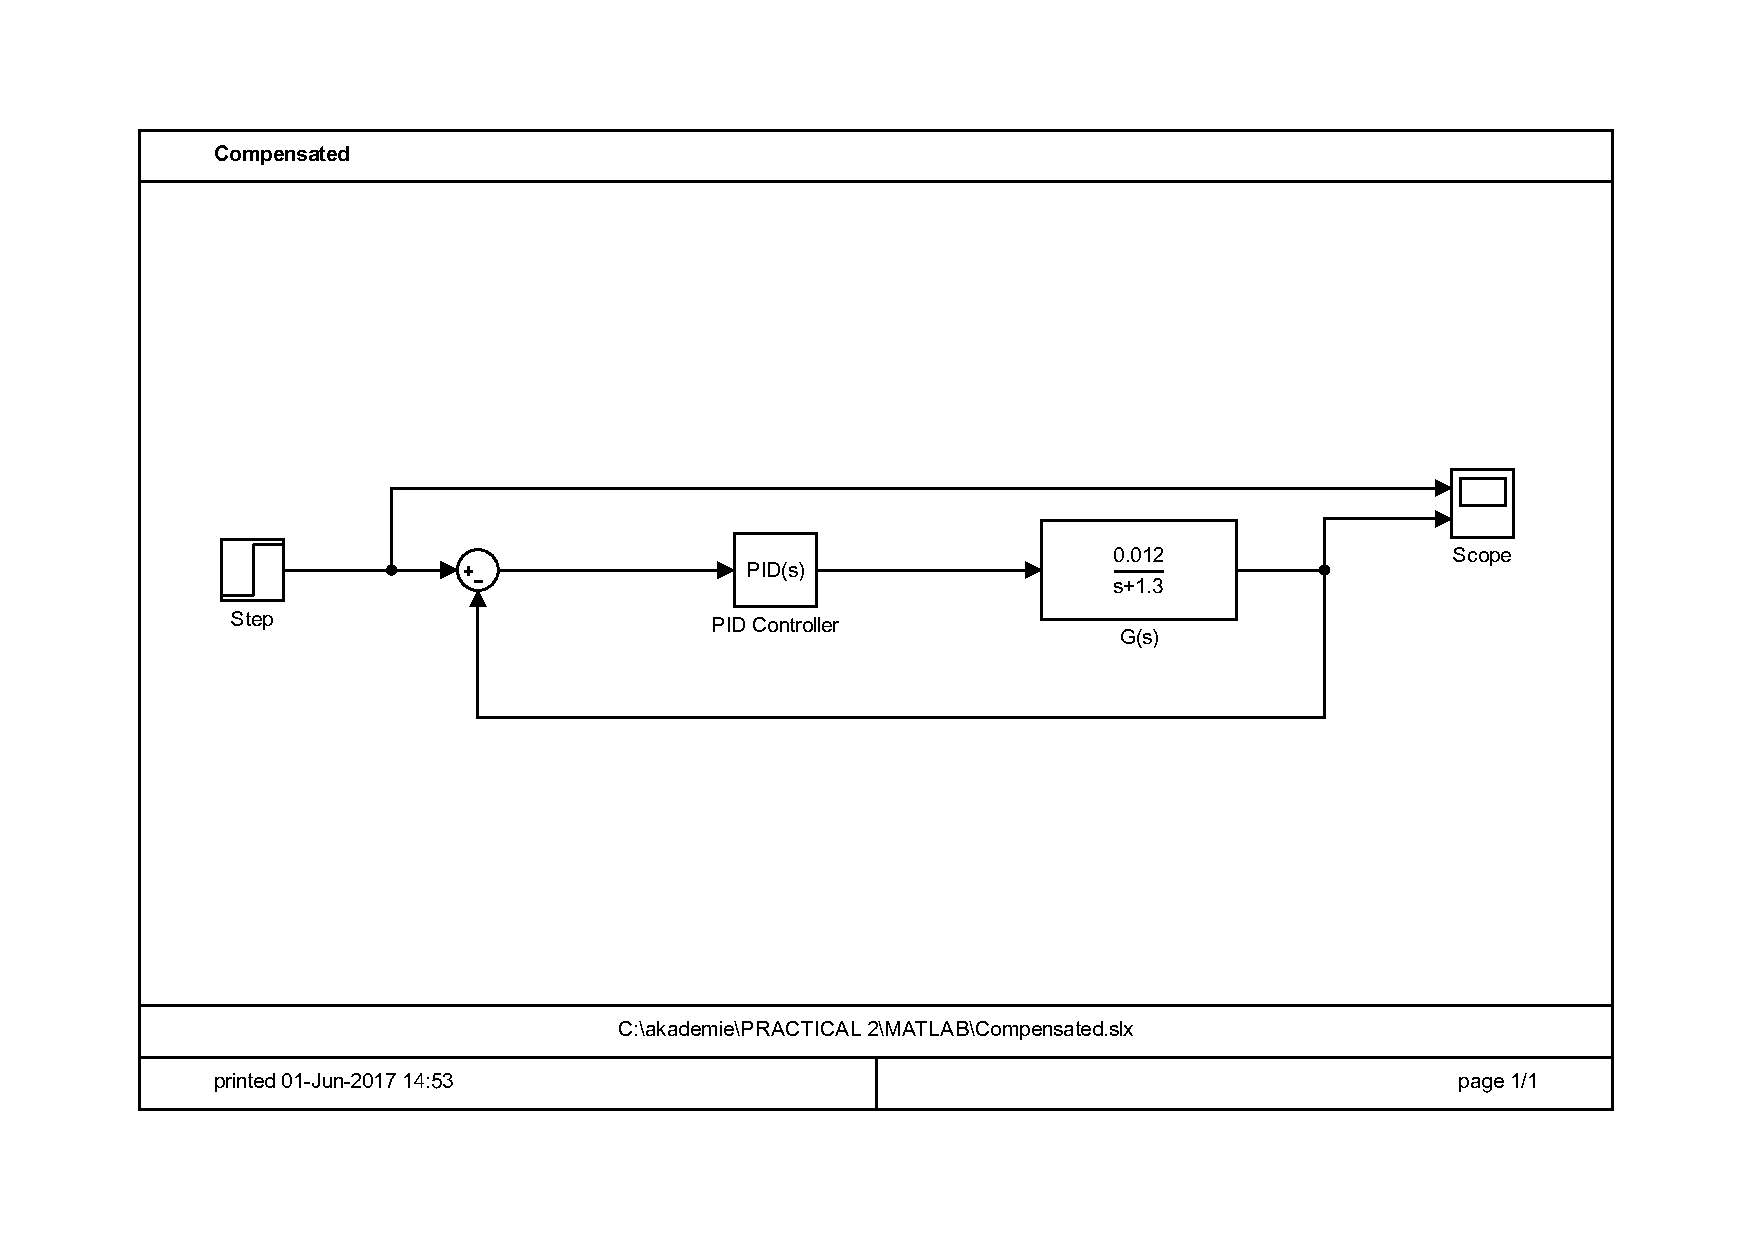
\includegraphics[clip,width=1\textwidth]{gfx/sim_Block_Diagram.pdf}%
		\caption{Simulink Block diagram of the compensated plant simulation }
\label{fig:simblockdiagram}
\end{figure}

The simulation in Figure~\ref{fig:simblockdiagram} yields the transient response in Figure~\ref{fig:simbtransplot}

\begin{figure}[h]
		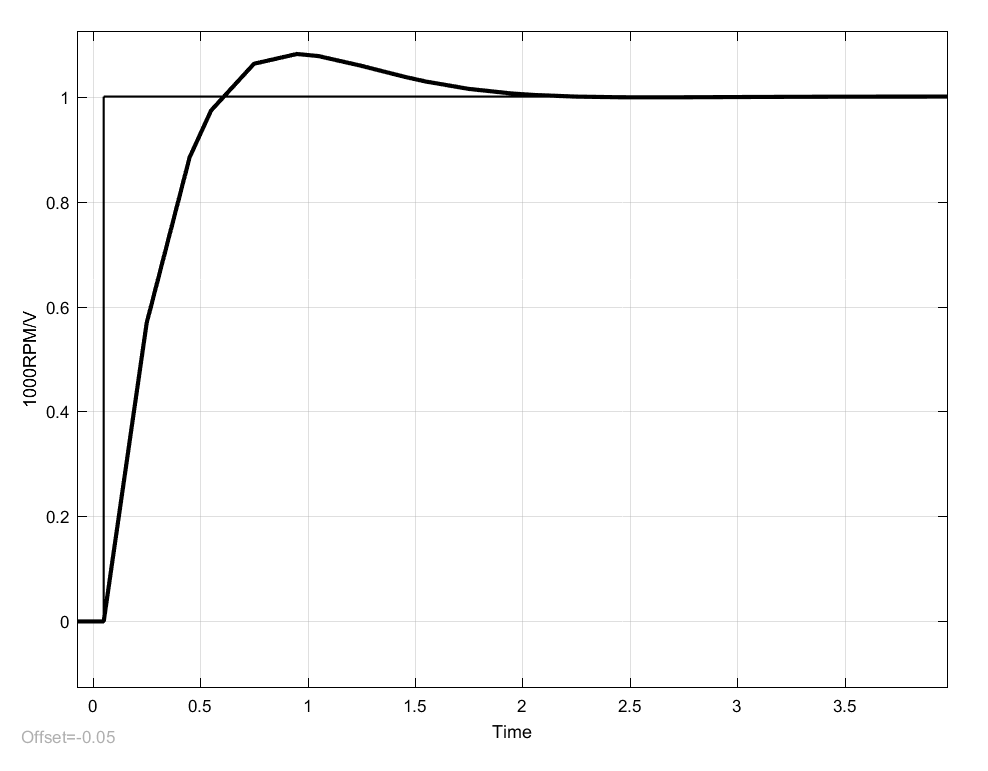
\includegraphics[clip,width=0.7\textwidth]{gfx/sim_plot}%
		\caption{Plot of the transient response of the simulated system}
\label{fig:simbtransplot}
\end{figure}

Table~\ref{tbl:simspec} Compares the specification to the simulated result of the calculated parameters:

\begin{table}[h]
\centering
\caption{Simulated Results}
\label{tbl:simspec}
\begin{tabular}{llll}
\cline{1-2}
\multicolumn{1}{|l|}{\textbf{Parameter}}      & \multicolumn{1}{l|}{\textbf{Value}} &  &  \\ \cline{1-2}
\multicolumn{1}{|l|}{Steady state error}    & \multicolumn{1}{l|}{0\%}                   &  &  \\ \cline{1-2}
\multicolumn{1}{|l|}{Percent Overshoot(P.O.)} & \multicolumn{1}{l|}{8.1 \%}                       &  &  \\ \cline{1-2}
\multicolumn{1}{|l|}{Settling time} & \multicolumn{1}{l|}{2s}                       &  &  \\ \cline{1-2}
                                              &                                             &  & 
\end{tabular}

\end{table}


\chapter{Practical Implementation}
Having calculated and simulated the PI compensator, it was implemented on an ARM microcontroller and connected to a driver circuit. The microcontroller was also configured to log the following data:
\begin{itemize}
	\item The desired set point (Volt)
	\item Tachometer output (Volt)
	\item Error (Volt)
	\item Duty cycle(\%)
\end{itemize}
The output used to plot Figure~\ref{fig:practrans} was prepared for plotting using the python script included in Appendix~\hyperref[apx:B]{B}. A step input of 1V was used, making the setpoint for the controller to track 1000RPM. 
\begin{figure}[h]
% GNUPLOT: LaTeX picture
\setlength{\unitlength}{0.240900pt}
\ifx\plotpoint\undefined\newsavebox{\plotpoint}\fi
\begin{picture}(1500,900)(0,0)
\sbox{\plotpoint}{\rule[-0.200pt]{0.400pt}{0.400pt}}%
\put(151.0,131.0){\rule[-0.200pt]{310.279pt}{0.400pt}}
\put(151.0,131.0){\rule[-0.200pt]{4.818pt}{0.400pt}}
\put(131,131){\makebox(0,0)[r]{$0$}}
\put(1419.0,131.0){\rule[-0.200pt]{4.818pt}{0.400pt}}
\put(151.0,252.0){\rule[-0.200pt]{310.279pt}{0.400pt}}
\put(151.0,252.0){\rule[-0.200pt]{4.818pt}{0.400pt}}
\put(131,252){\makebox(0,0)[r]{$0.2$}}
\put(1419.0,252.0){\rule[-0.200pt]{4.818pt}{0.400pt}}
\put(151.0,374.0){\rule[-0.200pt]{310.279pt}{0.400pt}}
\put(151.0,374.0){\rule[-0.200pt]{4.818pt}{0.400pt}}
\put(131,374){\makebox(0,0)[r]{$0.4$}}
\put(1419.0,374.0){\rule[-0.200pt]{4.818pt}{0.400pt}}
\put(151.0,495.0){\rule[-0.200pt]{310.279pt}{0.400pt}}
\put(151.0,495.0){\rule[-0.200pt]{4.818pt}{0.400pt}}
\put(131,495){\makebox(0,0)[r]{$0.6$}}
\put(1419.0,495.0){\rule[-0.200pt]{4.818pt}{0.400pt}}
\put(151.0,616.0){\rule[-0.200pt]{310.279pt}{0.400pt}}
\put(151.0,616.0){\rule[-0.200pt]{4.818pt}{0.400pt}}
\put(131,616){\makebox(0,0)[r]{$0.8$}}
\put(1419.0,616.0){\rule[-0.200pt]{4.818pt}{0.400pt}}
\put(151.0,738.0){\rule[-0.200pt]{310.279pt}{0.400pt}}
\put(151.0,738.0){\rule[-0.200pt]{4.818pt}{0.400pt}}
\put(131,738){\makebox(0,0)[r]{$1$}}
\put(1419.0,738.0){\rule[-0.200pt]{4.818pt}{0.400pt}}
\put(151.0,859.0){\rule[-0.200pt]{310.279pt}{0.400pt}}
\put(151.0,859.0){\rule[-0.200pt]{4.818pt}{0.400pt}}
\put(131,859){\makebox(0,0)[r]{$1.2$}}
\put(1419.0,859.0){\rule[-0.200pt]{4.818pt}{0.400pt}}
\put(151.0,131.0){\rule[-0.200pt]{0.400pt}{175.375pt}}
\put(151.0,131.0){\rule[-0.200pt]{0.400pt}{4.818pt}}
\put(151,90){\makebox(0,0){$0$}}
\put(151.0,839.0){\rule[-0.200pt]{0.400pt}{4.818pt}}
\put(409.0,131.0){\rule[-0.200pt]{0.400pt}{175.375pt}}
\put(409.0,131.0){\rule[-0.200pt]{0.400pt}{4.818pt}}
\put(409,90){\makebox(0,0){$2$}}
\put(409.0,839.0){\rule[-0.200pt]{0.400pt}{4.818pt}}
\put(666.0,131.0){\rule[-0.200pt]{0.400pt}{175.375pt}}
\put(666.0,131.0){\rule[-0.200pt]{0.400pt}{4.818pt}}
\put(666,90){\makebox(0,0){$4$}}
\put(666.0,839.0){\rule[-0.200pt]{0.400pt}{4.818pt}}
\put(924.0,131.0){\rule[-0.200pt]{0.400pt}{175.375pt}}
\put(924.0,131.0){\rule[-0.200pt]{0.400pt}{4.818pt}}
\put(924,90){\makebox(0,0){$6$}}
\put(924.0,839.0){\rule[-0.200pt]{0.400pt}{4.818pt}}
\put(1181.0,131.0){\rule[-0.200pt]{0.400pt}{175.375pt}}
\put(1181.0,131.0){\rule[-0.200pt]{0.400pt}{4.818pt}}
\put(1181,90){\makebox(0,0){$8$}}
\put(1181.0,839.0){\rule[-0.200pt]{0.400pt}{4.818pt}}
\put(1439.0,131.0){\rule[-0.200pt]{0.400pt}{175.375pt}}
\put(1439.0,131.0){\rule[-0.200pt]{0.400pt}{4.818pt}}
\put(1439,90){\makebox(0,0){$10$}}
\put(1439.0,839.0){\rule[-0.200pt]{0.400pt}{4.818pt}}
\put(151.0,131.0){\rule[-0.200pt]{0.400pt}{175.375pt}}
\put(151.0,131.0){\rule[-0.200pt]{310.279pt}{0.400pt}}
\put(1439.0,131.0){\rule[-0.200pt]{0.400pt}{175.375pt}}
\put(151.0,859.0){\rule[-0.200pt]{310.279pt}{0.400pt}}
\put(30,495){\makebox(0,0){\rotatebox{90}{Voltage/RPM}}}
\put(795,29){\makebox(0,0){Time}}
\put(151,201){\usebox{\plotpoint}}
\multiput(151.58,201.00)(0.493,0.853){23}{\rule{0.119pt}{0.777pt}}
\multiput(150.17,201.00)(13.000,20.387){2}{\rule{0.400pt}{0.388pt}}
\multiput(164.58,223.00)(0.493,0.695){23}{\rule{0.119pt}{0.654pt}}
\multiput(163.17,223.00)(13.000,16.643){2}{\rule{0.400pt}{0.327pt}}
\multiput(177.58,241.00)(0.493,0.933){23}{\rule{0.119pt}{0.838pt}}
\multiput(176.17,241.00)(13.000,22.260){2}{\rule{0.400pt}{0.419pt}}
\multiput(190.58,265.00)(0.493,0.933){23}{\rule{0.119pt}{0.838pt}}
\multiput(189.17,265.00)(13.000,22.260){2}{\rule{0.400pt}{0.419pt}}
\multiput(203.58,289.00)(0.492,1.056){21}{\rule{0.119pt}{0.933pt}}
\multiput(202.17,289.00)(12.000,23.063){2}{\rule{0.400pt}{0.467pt}}
\multiput(215.58,314.00)(0.493,1.012){23}{\rule{0.119pt}{0.900pt}}
\multiput(214.17,314.00)(13.000,24.132){2}{\rule{0.400pt}{0.450pt}}
\multiput(228.58,340.00)(0.493,0.972){23}{\rule{0.119pt}{0.869pt}}
\multiput(227.17,340.00)(13.000,23.196){2}{\rule{0.400pt}{0.435pt}}
\multiput(241.58,365.00)(0.493,3.431){23}{\rule{0.119pt}{2.777pt}}
\multiput(240.17,365.00)(13.000,81.236){2}{\rule{0.400pt}{1.388pt}}
\multiput(254.58,452.00)(0.493,1.052){23}{\rule{0.119pt}{0.931pt}}
\multiput(253.17,452.00)(13.000,25.068){2}{\rule{0.400pt}{0.465pt}}
\multiput(267.58,479.00)(0.493,1.091){23}{\rule{0.119pt}{0.962pt}}
\multiput(266.17,479.00)(13.000,26.004){2}{\rule{0.400pt}{0.481pt}}
\multiput(280.58,507.00)(0.493,1.131){23}{\rule{0.119pt}{0.992pt}}
\multiput(279.17,507.00)(13.000,26.940){2}{\rule{0.400pt}{0.496pt}}
\multiput(293.58,536.00)(0.493,1.091){23}{\rule{0.119pt}{0.962pt}}
\multiput(292.17,536.00)(13.000,26.004){2}{\rule{0.400pt}{0.481pt}}
\multiput(306.58,564.00)(0.492,1.272){21}{\rule{0.119pt}{1.100pt}}
\multiput(305.17,564.00)(12.000,27.717){2}{\rule{0.400pt}{0.550pt}}
\multiput(318.58,594.00)(0.493,1.171){23}{\rule{0.119pt}{1.023pt}}
\multiput(317.17,594.00)(13.000,27.877){2}{\rule{0.400pt}{0.512pt}}
\multiput(331.58,624.00)(0.493,1.131){23}{\rule{0.119pt}{0.992pt}}
\multiput(330.17,624.00)(13.000,26.940){2}{\rule{0.400pt}{0.496pt}}
\multiput(344.58,653.00)(0.493,1.131){23}{\rule{0.119pt}{0.992pt}}
\multiput(343.17,653.00)(13.000,26.940){2}{\rule{0.400pt}{0.496pt}}
\multiput(357.58,682.00)(0.493,0.655){23}{\rule{0.119pt}{0.623pt}}
\multiput(356.17,682.00)(13.000,15.707){2}{\rule{0.400pt}{0.312pt}}
\multiput(370.00,699.58)(0.497,0.493){23}{\rule{0.500pt}{0.119pt}}
\multiput(370.00,698.17)(11.962,13.000){2}{\rule{0.250pt}{0.400pt}}
\multiput(383.00,712.58)(0.652,0.491){17}{\rule{0.620pt}{0.118pt}}
\multiput(383.00,711.17)(11.713,10.000){2}{\rule{0.310pt}{0.400pt}}
\multiput(396.00,722.59)(0.728,0.489){15}{\rule{0.678pt}{0.118pt}}
\multiput(396.00,721.17)(11.593,9.000){2}{\rule{0.339pt}{0.400pt}}
\multiput(409.00,731.59)(0.758,0.488){13}{\rule{0.700pt}{0.117pt}}
\multiput(409.00,730.17)(10.547,8.000){2}{\rule{0.350pt}{0.400pt}}
\multiput(421.00,739.58)(0.590,0.492){19}{\rule{0.573pt}{0.118pt}}
\multiput(421.00,738.17)(11.811,11.000){2}{\rule{0.286pt}{0.400pt}}
\multiput(434.00,750.59)(1.123,0.482){9}{\rule{0.967pt}{0.116pt}}
\multiput(434.00,749.17)(10.994,6.000){2}{\rule{0.483pt}{0.400pt}}
\multiput(447.00,756.60)(1.797,0.468){5}{\rule{1.400pt}{0.113pt}}
\multiput(447.00,755.17)(10.094,4.000){2}{\rule{0.700pt}{0.400pt}}
\multiput(460.00,760.61)(2.695,0.447){3}{\rule{1.833pt}{0.108pt}}
\multiput(460.00,759.17)(9.195,3.000){2}{\rule{0.917pt}{0.400pt}}
\multiput(473.00,763.61)(2.695,0.447){3}{\rule{1.833pt}{0.108pt}}
\multiput(473.00,762.17)(9.195,3.000){2}{\rule{0.917pt}{0.400pt}}
\multiput(486.00,766.59)(1.378,0.477){7}{\rule{1.140pt}{0.115pt}}
\multiput(486.00,765.17)(10.634,5.000){2}{\rule{0.570pt}{0.400pt}}
\multiput(499.58,763.30)(0.493,-2.241){23}{\rule{0.119pt}{1.854pt}}
\multiput(498.17,767.15)(13.000,-53.152){2}{\rule{0.400pt}{0.927pt}}
\multiput(512.00,714.60)(1.797,0.468){5}{\rule{1.400pt}{0.113pt}}
\multiput(512.00,713.17)(10.094,4.000){2}{\rule{0.700pt}{0.400pt}}
\multiput(525.00,718.61)(2.472,0.447){3}{\rule{1.700pt}{0.108pt}}
\multiput(525.00,717.17)(8.472,3.000){2}{\rule{0.850pt}{0.400pt}}
\put(537,721.17){\rule{2.700pt}{0.400pt}}
\multiput(537.00,720.17)(7.396,2.000){2}{\rule{1.350pt}{0.400pt}}
\put(550,722.67){\rule{3.132pt}{0.400pt}}
\multiput(550.00,722.17)(6.500,1.000){2}{\rule{1.566pt}{0.400pt}}
\put(563,722.67){\rule{3.132pt}{0.400pt}}
\multiput(563.00,723.17)(6.500,-1.000){2}{\rule{1.566pt}{0.400pt}}
\put(589,723.17){\rule{2.700pt}{0.400pt}}
\multiput(589.00,722.17)(7.396,2.000){2}{\rule{1.350pt}{0.400pt}}
\put(576.0,723.0){\rule[-0.200pt]{3.132pt}{0.400pt}}
\put(628,723.67){\rule{2.891pt}{0.400pt}}
\multiput(628.00,724.17)(6.000,-1.000){2}{\rule{1.445pt}{0.400pt}}
\put(602.0,725.0){\rule[-0.200pt]{6.263pt}{0.400pt}}
\put(653,723.67){\rule{3.132pt}{0.400pt}}
\multiput(653.00,723.17)(6.500,1.000){2}{\rule{1.566pt}{0.400pt}}
\put(640.0,724.0){\rule[-0.200pt]{3.132pt}{0.400pt}}
\put(692,723.67){\rule{3.132pt}{0.400pt}}
\multiput(692.00,724.17)(6.500,-1.000){2}{\rule{1.566pt}{0.400pt}}
\put(705,723.67){\rule{3.132pt}{0.400pt}}
\multiput(705.00,723.17)(6.500,1.000){2}{\rule{1.566pt}{0.400pt}}
\put(718,724.67){\rule{3.132pt}{0.400pt}}
\multiput(718.00,724.17)(6.500,1.000){2}{\rule{1.566pt}{0.400pt}}
\put(731,725.67){\rule{2.891pt}{0.400pt}}
\multiput(731.00,725.17)(6.000,1.000){2}{\rule{1.445pt}{0.400pt}}
\put(743,726.67){\rule{3.132pt}{0.400pt}}
\multiput(743.00,726.17)(6.500,1.000){2}{\rule{1.566pt}{0.400pt}}
\put(756,726.67){\rule{3.132pt}{0.400pt}}
\multiput(756.00,727.17)(6.500,-1.000){2}{\rule{1.566pt}{0.400pt}}
\put(769,725.67){\rule{3.132pt}{0.400pt}}
\multiput(769.00,726.17)(6.500,-1.000){2}{\rule{1.566pt}{0.400pt}}
\put(782,724.67){\rule{3.132pt}{0.400pt}}
\multiput(782.00,725.17)(6.500,-1.000){2}{\rule{1.566pt}{0.400pt}}
\put(795,724.67){\rule{3.132pt}{0.400pt}}
\multiput(795.00,724.17)(6.500,1.000){2}{\rule{1.566pt}{0.400pt}}
\put(808,725.67){\rule{3.132pt}{0.400pt}}
\multiput(808.00,725.17)(6.500,1.000){2}{\rule{1.566pt}{0.400pt}}
\put(821,726.67){\rule{3.132pt}{0.400pt}}
\multiput(821.00,726.17)(6.500,1.000){2}{\rule{1.566pt}{0.400pt}}
\put(834,727.67){\rule{3.132pt}{0.400pt}}
\multiput(834.00,727.17)(6.500,1.000){2}{\rule{1.566pt}{0.400pt}}
\put(666.0,725.0){\rule[-0.200pt]{6.263pt}{0.400pt}}
\put(859,728.67){\rule{3.132pt}{0.400pt}}
\multiput(859.00,728.17)(6.500,1.000){2}{\rule{1.566pt}{0.400pt}}
\put(872,729.67){\rule{3.132pt}{0.400pt}}
\multiput(872.00,729.17)(6.500,1.000){2}{\rule{1.566pt}{0.400pt}}
\put(885,731.17){\rule{2.700pt}{0.400pt}}
\multiput(885.00,730.17)(7.396,2.000){2}{\rule{1.350pt}{0.400pt}}
\put(898,733.17){\rule{2.700pt}{0.400pt}}
\multiput(898.00,732.17)(7.396,2.000){2}{\rule{1.350pt}{0.400pt}}
\put(847.0,729.0){\rule[-0.200pt]{2.891pt}{0.400pt}}
\put(937,734.67){\rule{3.132pt}{0.400pt}}
\multiput(937.00,734.17)(6.500,1.000){2}{\rule{1.566pt}{0.400pt}}
\put(950,736.17){\rule{2.500pt}{0.400pt}}
\multiput(950.00,735.17)(6.811,2.000){2}{\rule{1.250pt}{0.400pt}}
\put(962,737.67){\rule{3.132pt}{0.400pt}}
\multiput(962.00,737.17)(6.500,1.000){2}{\rule{1.566pt}{0.400pt}}
\put(975,738.67){\rule{3.132pt}{0.400pt}}
\multiput(975.00,738.17)(6.500,1.000){2}{\rule{1.566pt}{0.400pt}}
\put(988,738.67){\rule{3.132pt}{0.400pt}}
\multiput(988.00,739.17)(6.500,-1.000){2}{\rule{1.566pt}{0.400pt}}
\put(911.0,735.0){\rule[-0.200pt]{6.263pt}{0.400pt}}
\put(1014,738.67){\rule{3.132pt}{0.400pt}}
\multiput(1014.00,738.17)(6.500,1.000){2}{\rule{1.566pt}{0.400pt}}
\put(1001.0,739.0){\rule[-0.200pt]{3.132pt}{0.400pt}}
\put(1053,738.67){\rule{2.891pt}{0.400pt}}
\multiput(1053.00,739.17)(6.000,-1.000){2}{\rule{1.445pt}{0.400pt}}
\put(1065,737.67){\rule{3.132pt}{0.400pt}}
\multiput(1065.00,738.17)(6.500,-1.000){2}{\rule{1.566pt}{0.400pt}}
\put(1078,737.67){\rule{3.132pt}{0.400pt}}
\multiput(1078.00,737.17)(6.500,1.000){2}{\rule{1.566pt}{0.400pt}}
\put(1091,737.67){\rule{3.132pt}{0.400pt}}
\multiput(1091.00,738.17)(6.500,-1.000){2}{\rule{1.566pt}{0.400pt}}
\put(1104,736.67){\rule{3.132pt}{0.400pt}}
\multiput(1104.00,737.17)(6.500,-1.000){2}{\rule{1.566pt}{0.400pt}}
\put(1117,735.67){\rule{3.132pt}{0.400pt}}
\multiput(1117.00,736.17)(6.500,-1.000){2}{\rule{1.566pt}{0.400pt}}
\put(1027.0,740.0){\rule[-0.200pt]{6.263pt}{0.400pt}}
\put(1143,734.17){\rule{2.700pt}{0.400pt}}
\multiput(1143.00,735.17)(7.396,-2.000){2}{\rule{1.350pt}{0.400pt}}
\put(1156,732.67){\rule{3.132pt}{0.400pt}}
\multiput(1156.00,733.17)(6.500,-1.000){2}{\rule{1.566pt}{0.400pt}}
\put(1130.0,736.0){\rule[-0.200pt]{3.132pt}{0.400pt}}
\put(1207,731.17){\rule{2.700pt}{0.400pt}}
\multiput(1207.00,732.17)(7.396,-2.000){2}{\rule{1.350pt}{0.400pt}}
\put(1220,729.67){\rule{3.132pt}{0.400pt}}
\multiput(1220.00,730.17)(6.500,-1.000){2}{\rule{1.566pt}{0.400pt}}
\put(1233,728.17){\rule{2.700pt}{0.400pt}}
\multiput(1233.00,729.17)(7.396,-2.000){2}{\rule{1.350pt}{0.400pt}}
\put(1246,727.67){\rule{3.132pt}{0.400pt}}
\multiput(1246.00,727.17)(6.500,1.000){2}{\rule{1.566pt}{0.400pt}}
\put(1259,728.67){\rule{3.132pt}{0.400pt}}
\multiput(1259.00,728.17)(6.500,1.000){2}{\rule{1.566pt}{0.400pt}}
\put(1272,728.17){\rule{2.500pt}{0.400pt}}
\multiput(1272.00,729.17)(6.811,-2.000){2}{\rule{1.250pt}{0.400pt}}
\put(1169.0,733.0){\rule[-0.200pt]{9.154pt}{0.400pt}}
\put(1323,726.67){\rule{3.132pt}{0.400pt}}
\multiput(1323.00,727.17)(6.500,-1.000){2}{\rule{1.566pt}{0.400pt}}
\put(1336,725.67){\rule{3.132pt}{0.400pt}}
\multiput(1336.00,726.17)(6.500,-1.000){2}{\rule{1.566pt}{0.400pt}}
\put(1349,726.17){\rule{2.700pt}{0.400pt}}
\multiput(1349.00,725.17)(7.396,2.000){2}{\rule{1.350pt}{0.400pt}}
\put(1362,727.67){\rule{3.132pt}{0.400pt}}
\multiput(1362.00,727.17)(6.500,1.000){2}{\rule{1.566pt}{0.400pt}}
\put(1284.0,728.0){\rule[-0.200pt]{9.395pt}{0.400pt}}
\put(1387,727.67){\rule{3.132pt}{0.400pt}}
\multiput(1387.00,728.17)(6.500,-1.000){2}{\rule{1.566pt}{0.400pt}}
\put(1375.0,729.0){\rule[-0.200pt]{2.891pt}{0.400pt}}
\put(1413,727.67){\rule{3.132pt}{0.400pt}}
\multiput(1413.00,727.17)(6.500,1.000){2}{\rule{1.566pt}{0.400pt}}
\put(1426,727.67){\rule{3.132pt}{0.400pt}}
\multiput(1426.00,728.17)(6.500,-1.000){2}{\rule{1.566pt}{0.400pt}}
\put(1400.0,728.0){\rule[-0.200pt]{3.132pt}{0.400pt}}
\put(1439,728){\usebox{\plotpoint}}
\put(151.0,131.0){\rule[-0.200pt]{0.400pt}{175.375pt}}
\put(151.0,131.0){\rule[-0.200pt]{310.279pt}{0.400pt}}
\put(1439.0,131.0){\rule[-0.200pt]{0.400pt}{175.375pt}}
\put(151.0,859.0){\rule[-0.200pt]{310.279pt}{0.400pt}}
\end{picture}

\caption{Practical measurement, transient step response}
	\label{fig:practrans}
\end{figure}
Table~\ref{tbl:measspec} shows the practical results.
\begin{table}[h]
\centering
\caption{Simulated Results}
\label{tbl:measspec}
\begin{tabular}{llll}
\cline{1-2}
\multicolumn{1}{|l|}{\textbf{Parameter}}      & \multicolumn{1}{l|}{\textbf{Value}} &  &  \\ \cline{1-2}
\multicolumn{1}{|l|}{Steady state error}    & \multicolumn{1}{l|}{3\%}                   &  &  \\ \cline{1-2}
\multicolumn{1}{|l|}{Percent Overshoot(P.O.)} & \multicolumn{1}{l|}{7.1 \%}                       &  &  \\ \cline{1-2}
\multicolumn{1}{|l|}{Settling time} & \multicolumn{1}{l|}{6s}                       &  &  \\ \cline{1-2}
                                              &                                             &  & 
\end{tabular}

\end{table}


\chapter{Results}
%table comparing P.O, Ts Es etc for calc, sim and prac. 
\begin{table}[h]
\centering
\caption{Compiled Results}
\begin{tabular}{|l|l|l|l|l}
\cline{1-4}
                             & P.O    & $E_{ss}$ & $T_s$       &  \\ \cline{1-4}
\textbf{Specification}       & 10\%   & 1\%      & \textless2s &  \\ \cline{1-4}
\textbf{Calculation Results} & 10.5\% & 0\%      & 2.2s        &  \\ \cline{1-4}
\textbf{Simulation Results}  & 8.1\%  & 0\%      & 2s          &  \\ \cline{1-4}
\textbf{Practical Results}   & 7.1\%  & 3\%      & 2.5s        &  \\ \cline{1-4}
\end{tabular}


\end{table}

\chapter{Discussion of results and Conclusion}
The calculations, simulation and practical measurements all performed within a reasonable margin from the specifications. The steady state error in the practical measurements is due to inaccuracies in the measuring equipment and other environmental factors. The assignment was very educational and provided insights to a full stack controller implementation.



